\section{评估}
\label{sec:evaluation}

本节对 \sysname 进行全面评估，覆盖整体训练性能（\S\ref{sec:evaluation:performance}）、\sysname 关键优化的消融研究（\S\ref{sec:evaluation:ablation}），以及精度-通信协同设计的有效性（\S\ref{sec:evaluation:co-design}）。表~\ref{tab:evaluation:model_conf} 列出了评估中使用的 MoE 模型配置，包括隐藏维度（$h$）、FFN 中间维度（$h_{ffn}$）、专家数量以及 top-$k$ 值。
除非另有说明，评估均在 NVIDIA H800 GPU 上进行，其规格见 表~\ref{tab:evaluation:gpu_spec}。

\begin{table}[t!]
    \centering
    \resizebox{\linewidth}{!} {
        \begin{tabular}{c|c|c|c|c}
            \hline
            \hline
            \multirow{2}{*}{\begin{tabular}[c]{@{}c@{}}系统\end{tabular}} & \multirow{2}{*}{\begin{tabular}[c]{@{}c@{}}\#GPU\end{tabular}} & \multirow{2}{*}{\begin{tabular}[c]{@{}c@{}}迭代\\ 时间 (s)\end{tabular}} & \multirow{2}{*}{\begin{tabular}[c]{@{}c@{}}吞吐\\ (tokens/s)\end{tabular}} & \multirow{2}{*}{\begin{tabular}[c]{@{}c@{}}训练 1T tokens\\ 所需时间 (天)\end{tabular}} \\
            & & & & \\\cline{1-5}
            \multirow{5}{*}{Megatron-LM} & 240 & 39.94 & 151.1k & 76.61 \\
            & 480 & 19.56 & 301.1k & 38.38 \\
            & 720 & 13.70 & 430.5k & 26.88 \\
            & 960 & 10.82 & 550.2k & 21.23 \\
            & 1440 & 7.90 & 746.6k & 15.50 \\\cline{1-5}
            \multirow{5}{*}{\sysname} & 240 & 21.61 & 272.9k (\textbf{1.81$\times$}) & 42.41 \\
            & 480 & 11.83 & 498.6k (\textbf{1.65$\times$}) & 23.21 \\
            & 720 & 7.97 & 740.1k (\textbf{1.72$\times$}) & 15.64 \\
            & 960 & 6.12 & 963.8k (\textbf{1.77$\times$}) & 12.01 \\
            & 1440 & 4.19 & 1407.7k (\textbf{1.88$\times$}) & 8.22 \\
            \hline
            \hline
        \end{tabular}
    }
    % \vspace{-0.1in}
    \caption{使用 NVIDIA H800 GPU 训练 352B MoE 模型的强扩展性能。吞吐列括号中的数字表示 \sysname 相比 Megatron-LM 的加速比。}
    \vspace{-0.2in}
    \label{tab:evaluation:strong-scaling}
\end{table}

\subsection{训练性能}
\label{sec:evaluation:performance}

\sysname 构建在 Megatron-LM~\cite{shoeybi2019megatron} 之上。Megatron-LM 是最先进的开源 LLM 训练系统之一，支持 3D 并行策略，并持续吸收社区最新优化。我们的评估使用 GitHub 上 commit hash 为 f1f03922 的 Megatron-LM~\cite{megatron-lm}，选择该版本是因为它在数月前实验开始时较为稳定。为公平比较，我们对 Megatron-LM 和 \sysname 使用相同的全局 batch size，并分别为两个系统选择最优并行配置。具体而言，\sysname 在每个节点内采用 SP attention 和 EP，而 Megatron-LM 在每个节点内采用 TP；两个系统都配置 PP size 为 15。\revision{我们调优 Megatron-LM 的配置，以满足其要求所有组件使用统一 TP size 的限制。如 \S\ref{sec:design:parallelism:sp_attention} 所讨论，对于 Megatron-LM，TP size 为 1 会导致无法接受的 8$\times$ 激活内存（只能通过缓慢的 gradient checkpointing 重算来处理），而 TP size 为 8 又会迫使 EP 跨节点运行，产生比 PP 更高的通信成本。值得注意的是，评估中的两个系统都启用了 MegaScale~\cite{jiang2024megascale} 中用于数据并行和流水线并行的通信-计算重叠技术。因此，通信开销主要来自节点内模型并行，例如 TP、SP 和 EP。} 序列长度为 8,192，词表大小为 65,536。
% \todo{Can we mention the hardware used in the experiments? e.g., Hopper GPUs? Unclear what GPUs Table 3 and Figure 11 use. Only Figure 12 has the GPU types.}

% \begin{table}[t!]
%     \centering
%     \resizebox{\linewidth}{!} {
%         \begin{tabular}{c|c|c|c|c}
%             \hline
%             \hline
%             \multirow{2}{*}{\begin{tabular}[c]{@{}c@{}}System\end{tabular}} & \multirow{2}{*}{\begin{tabular}[c]{@{}c@{}}\#GPUs\end{tabular}} & \multirow{2}{*}{\begin{tabular}[c]{@{}c@{}}Iteration\\ Time (s)\end{tabular}} & \multirow{2}{*}{\begin{tabular}[c]{@{}c@{}}Throughput\\ (tokens/s)\end{tabular}} & \multirow{2}{*}{\begin{tabular}[c]{@{}c@{}}MFU\end{tabular}} \\
%             & & & & \\\cline{1-5}
%             \multirow{5}{*}{Megatron-LM} & 240 & 39.94 & 151.1k & 17.98\% \\
%             & 480 & 19.56 & 301.1k & 17.94\% \\
%             & 720 & 13.70 & 430.5k & 17.08\% \\
%             & 960 & 10.82 & 550.2k & 16.22\% \\
%             & 1440 & 7.90 & 746.6k & 14.81\% \\\cline{1-5}
%             \multirow{5}{*}{\sysname} & 240 & 21.61 & 272.9k & 32.48\%(\textbf{1.81$\times$}) \\
%             & 480 & 11.83 & 498.6k & 29.67\% (\textbf{1.65$\times$}) \\
%             & 720 & 7.97 & 740.1k & 29.36\% (\textbf{1.72$\times$}) \\
%             & 960 & 6.12 & 963.8k & 28.67\% (\textbf{1.77$\times$}) \\
%             & 1440 & 4.19 & 1407.7k & 27.89\% (\textbf{1.88$\times$}) \\
%             \hline
%             \hline
%         \end{tabular}
%     }
%     % \vspace{0.05in}
%     \caption{Strong-scaling training performance for the 352B MoE model, with a global batch size of 720 for all experiments. The number in parentheses in the MFU column represents the speedup of \sysname compared to Megatron-LM.}
%     \vspace{-0.15in}
%     \label{tab:evaluation:strong-scaling}
% \end{table}

% \begin{table*}[t!]
%     \centering
%     \resizebox{\linewidth}{!} {
%         \begin{tabular}{c|c|c|c|c|c|c}
%             \hline
%             \hline
%             \multirow{2}{*}{\begin{tabular}[c]{@{}c@{}}Batch Size\end{tabular}} & \multirow{2}{*}{\begin{tabular}[c]{@{}c@{}}System\end{tabular}} & \multirow{2}{*}{\begin{tabular}[c]{@{}c@{}}\#GPUs\end{tabular}} & \multirow{2}{*}{\begin{tabular}[c]{@{}c@{}}Iteration Time (s)\end{tabular}} & \multirow{2}{*}{\begin{tabular}[c]{@{}c@{}}Throughput\\ (tokens/s)\end{tabular}} & \multirow{2}{*}{\begin{tabular}[c]{@{}c@{}}MFU\end{tabular}} & \multirow{2}{*}{\begin{tabular}[c]{@{}c@{}}Aggregated\\ PFlops/s\end{tabular}}  \\
%             & & & & & & \\\cline{1-7}
%             \multirow{10}{*}{720} 
%             & \multirow{5}{*}{Megatron-LM} & 240 & 39.94 & 151.1k & 17.98\% & 42.68 \\
%             &  & 480 & 19.56 & 301.1k & 17.94\% & 85.16 \\
%             &  & 720 & 13.70 & 430.5k & 17.08\% & 121.62 \\
%             &  & 960 & 10.72 & 550.2k & 16.37\% & 155.42 \\
%             &  & 1440 & 7.90 & 746.6k & 14.81\% & 210.92 \\\cline{2-7}
%             & \multirow{5}{*}{\sysname} & 240 & 21.61 & 272.9k & 32.48\%(\textbf{1.81$\times$}) & 77.09 \\
%             &  & 480 & 11.83 & 498.6k & 29.67\% (\textbf{1.65$\times$}) & 140.85 \\
%             &  & 720 & 7.97 & 7401.k & 29.36\% (\textbf{1.72$\times$}) & 209.07 \\
%             &  & 960 & 6.12 & 963.8k & 28.67\% (\textbf{1.75$\times$}) & 272.20 \\
%             &  & 1440 & 4.19 & 1407.7k & 27.89\% (\textbf{1.88$\times$}) & 397.20 \\
%             \hline
%             \hline
%         \end{tabular}
%     }
%     \caption{Strong-scaling training performance for the 352B MoE model. The number in parentheses in the MFU column represents the speedup of \sysname compared to Megatron-LM. \todo{More details in the title. Refer to MegaScale.}}
%     \vspace{-0.15in}
%     \label{tab:evaluation:scalability}
% \end{table*}

\begin{figure}[t!]
    \centering
    
\includegraphics[width=0.8\linewidth]{figures/eval/weak_scaling.pdf}
    \vspace{-0.15in}
    \caption{使用 NVIDIA H800 GPU 训练 352B MoE 模型的弱扩展性能。}
    \vspace{-0.1in}
    \label{fig:eval:weak-scaling}
\end{figure}

\parabf{可扩展性。} 表~\ref{tab:evaluation:strong-scaling} 比较了 Megatron-LM 和 \sysname 在 352B MoE 模型上的强扩展训练性能。我们在保持全局 batch size 固定为 720 的情况下扩展 GPU 数量。
% This experimental setting is more realistic, given that batch size is constrained by convergence effects and cannot be indefinitely scaled with the number of GPUs. 
在所有设置下，\sysname 相比 Megatron-LM 实现 1.65--1.88$\times$ 加速。随着 GPU 数量增加，\sysname 的 MFU（Model FLOPs Utilization）从 32.48\% 下降到 27.89\%。这是预期现象，因为 batch size 固定，而随着 GPU 增多，每条流水线的 micro-batch 数量减少，从而产生更多气泡。

图~\ref{fig:eval:weak-scaling} 展示了 Megatron-LM 和 \sysname 在同一模型上的弱扩展训练性能。我们按 GPU 数量（从 480 到 1,440）等比例将全局 batch size 从 360 扩展到 1,080。相比 Megatron-LM，\sysname 实现了 1.74--1.79$\times$ 的训练吞吐。随着规模增大，Megatron-LM 因通信开销增加而吞吐下降 2.74\%。相比之下，\sysname 受益于全面的通信-计算重叠，表现出近线性扩展性，吞吐仅下降 0.2\%。
% \sysname achieves a 12.67\% higher MFU than Megatron-LM. As the scale increases, Megatron-LM’s MFU drops by 0.46\% due to increased communication overhead, whereas \sysname exhibits near-linear scalability, benefiting from comprehensive communication overlap. 

\begin{figure}[t!]
    \centering
    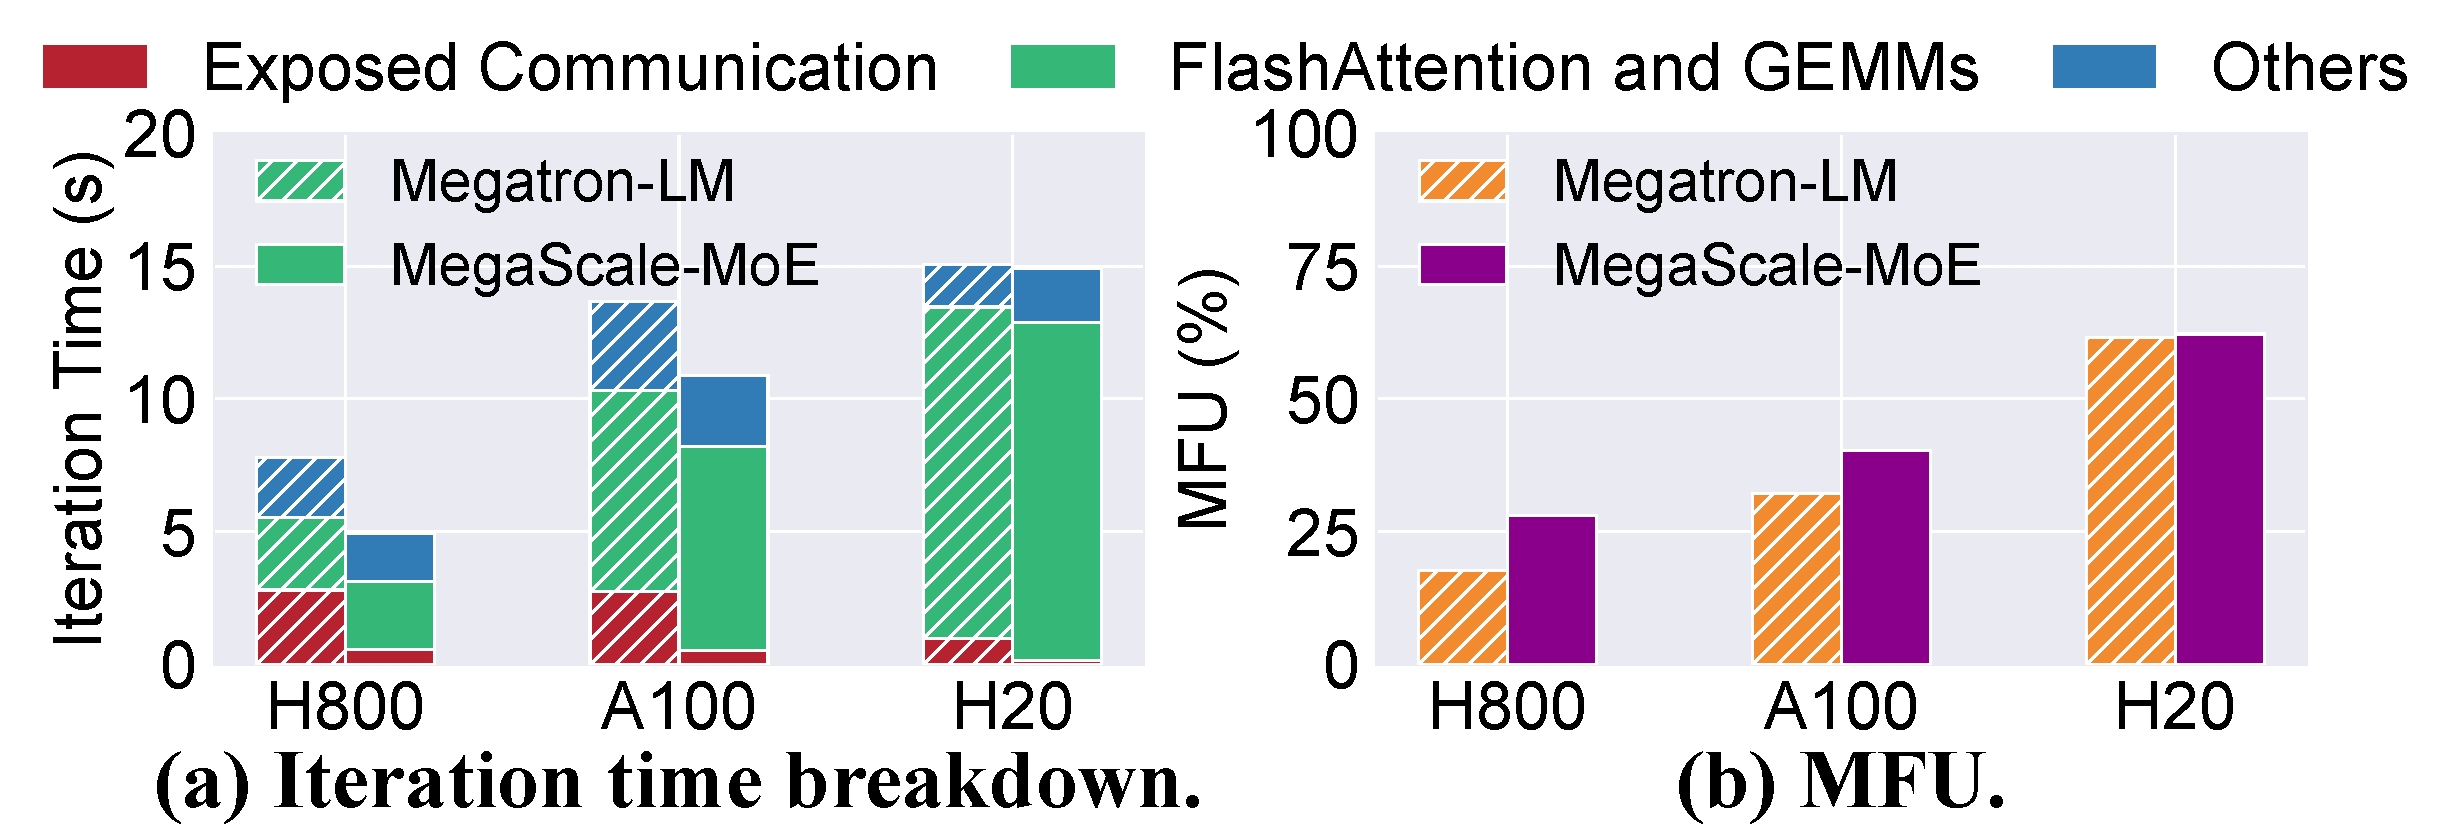
\includegraphics[width=\linewidth]{figures/eval/different_gpus.pdf}
    \vspace{-0.3in}
    \caption{在不同 GPU 上训练 Mixtral-8$\times$7B 的性能分解。}
    \vspace{-0.1in}
    \label{fig:eval:different_gpus}
\end{figure}

\begin{table}[t!]
    \centering
    \resizebox{0.9\linewidth}{!} {
        \begin{tabular}{c|c|c|c|c}
            \hline
            % \hline
            \multirow{2}{*}{GPU} & 
            \multirow{2}{*}{\begin{tabular}[c]{@{}c@{}}计算能\\力 (TFLOPS)\end{tabular}} & 
            \multicolumn{2}{c|}{内存规格} & 
            \multirow{2}{*}{\begin{tabular}[c]{@{}c@{}}NVLink\\ Bw. (GB/s)\end{tabular}} \\
            \cline{3-4}
            & & 容量 (GB) & 带宽 (TB/s) & \\
            \hline
            H800 & 989 & 80 & 3.4 & 400 \\
            A100 & 312 & 80 & 2.0 & 600 \\
            H20 & 148 & 96 & 4.0 & 900 \\
            \hline
            % \hline
        \end{tabular}
    }
    % \vspace{-0.1in}
    \caption{不同 NVIDIA GPU 的规格。}
    \vspace{-0.15in}
    \label{tab:evaluation:gpu_spec}
\end{table}

\parabf{不同 GPU 上的性能分解。} 为进一步理解生产环境中训练 MoE 模型的性能，我们对 \sysname 进行了深入分析。我们分别在 32 张 NVIDIA H800、H20 和 A100 GPU 上训练 Mixtral-8$\times$7B。所用 GPU 的规格列于 表~\ref{tab:evaluation:gpu_spec}。我们将 DP size 设为 4，Megatron-LM 的 TP size 设为 8，\sysname 的 SP 和 EP size 设为 8。如 图~\ref{fig:eval:different_gpus}b 所示，在这些 GPU 上，\sysname 在 MFU 上始终优于 Megatron-LM，最高达到 1.58$\times$。
图~\ref{fig:eval:different_gpus}a 展示了 Megatron-LM 和 \sysname 的迭代时间分解。暴露通信时间表示未与计算操作重叠的通信时间。FlashAttention 和 GEMM 是我们计算 MFU 时统计的操作。性能提升主要来自 \sysname 的通信高效并行策略和细粒度重叠通信。

需要注意，随着 GPU 计算能力增强，MFU 数值会下降。这是因为不同于稠密模型，MoE 模型包含许多内存密集型操作，如 routing、本地 scatter 和 gather；由于内存带宽并未像计算能力一样快速增长，这些操作仍然耗时。此外，GEMM 效率也会随计算能力提高而下降，因为它同样依赖受内存带宽约束的内存加载。

\subsection{消融研究}
\label{sec:evaluation:ablation}

\begin{table}[t!]
    \centering
    \resizebox{\linewidth}{!} {
        \begin{tabular}{c|c|c|c}
            \hline
            \hline
            \multirow{2}{*}{\begin{tabular}[c]{@{}c@{}}编号\end{tabular}} & \multirow{2}{*}{\begin{tabular}[c]{@{}c@{}}方法\end{tabular}} & \multirow{2}{*}{\begin{tabular}[c]{@{}c@{}}归一化\\ 吞吐\end{tabular}} & \multirow{2}{*}{\begin{tabular}[c]{@{}c@{}} $\Delta$ \end{tabular}} \\
            & & & \\\cline{1-4}
            1 & baseline & 1 & \\
            2 & (1) 加 SP+EP & 1.13 & +13\% \\
            3 & (2) 加算子间重叠 & 1.22 & +9\% \\
            4 & (3) 加算子内重叠 & 1.28 & +6\% \\
            \hline
            \hline
        \end{tabular}
    }
    % \vspace{-0.1in}
    \caption{\revision{使用 240 张 NVIDIA H800 GPU、batch size 为 720 训练 352B MoE 模型时的吞吐提升分解。}}
    \vspace{-0.2in}
    \label{tab:evaluation:systematic_ablation}
\end{table}

\revision{我们评估 \sysname 各项优化技术的有效性。首先，我们通过逐步启用每项技术进行系统性分解实验，以隔离其对整体性能的贡献。表~\ref{tab:evaluation:systematic_ablation} 展示了在 240 张 GPU 上以全局 batch size 720 训练 352B MoE 模型时，不同优化带来的吞吐提升分解。baseline 是 \sysname 的一个版本，它对注意力和 FFN 都采用 TP，并禁用通信-计算重叠。首先，通过应用通信高效策略，即对注意力采用 SP、对专家采用 EP，我们相对该 baseline 获得初始 13\% 的吞吐提升。随后，我们针对大规模 MoE 训练中的主要瓶颈，即通信开销。我们的算子间和算子内重叠方法有效隐藏这些成本，分别进一步带来额外 9\% 和 6\% 的训练加速。}

\begin{figure}[t!]
    \centering
    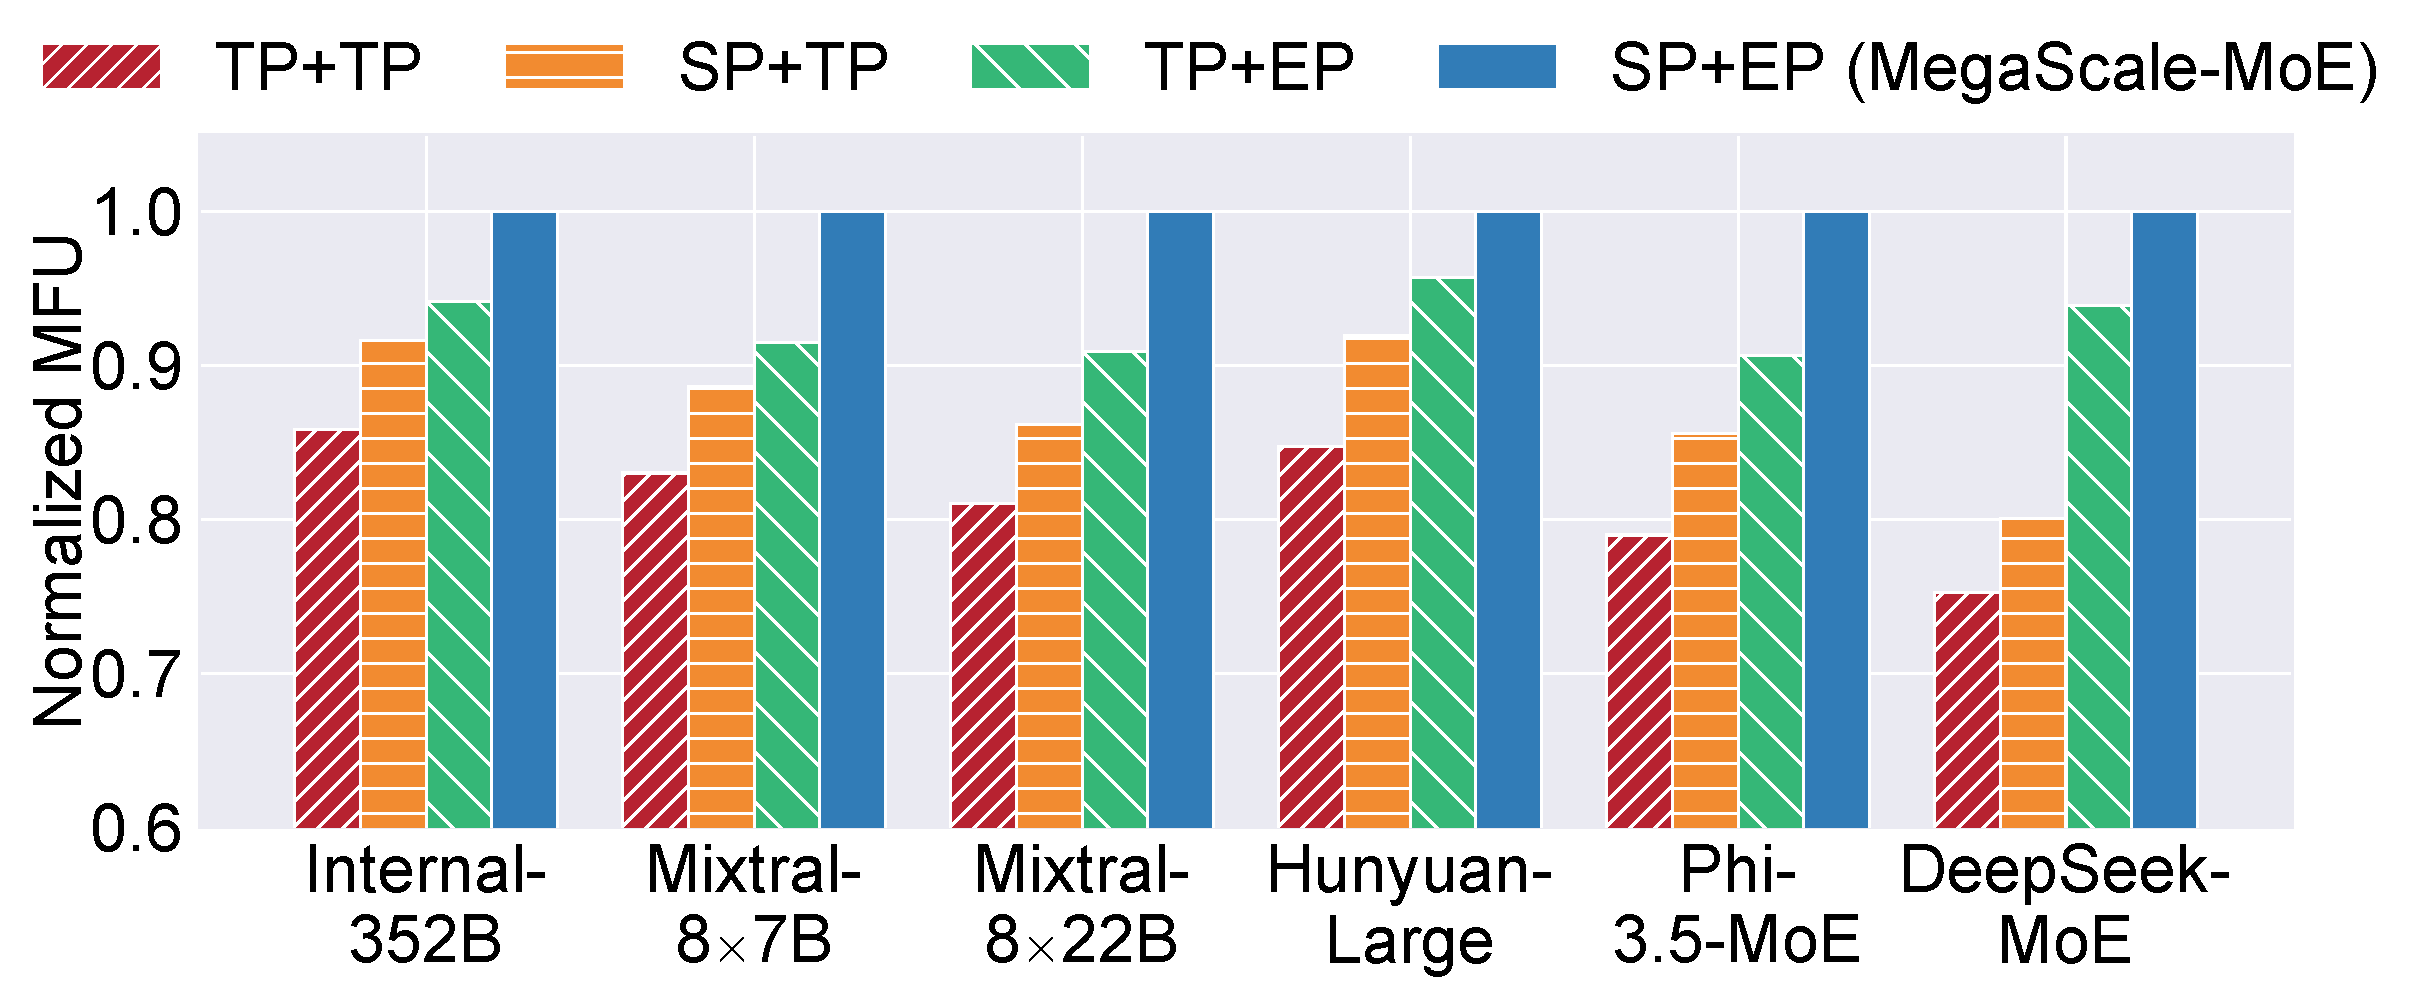
\includegraphics[width=0.8\linewidth]{figures/eval/parallelism_efficiency.pdf}
    \vspace{-0.15in}
    \caption{不同模型的并行效率。}
    \vspace{-0.1in}
    \label{fig:eval:parallelism}
\end{figure}

\begin{figure}[t!]
    \centering
    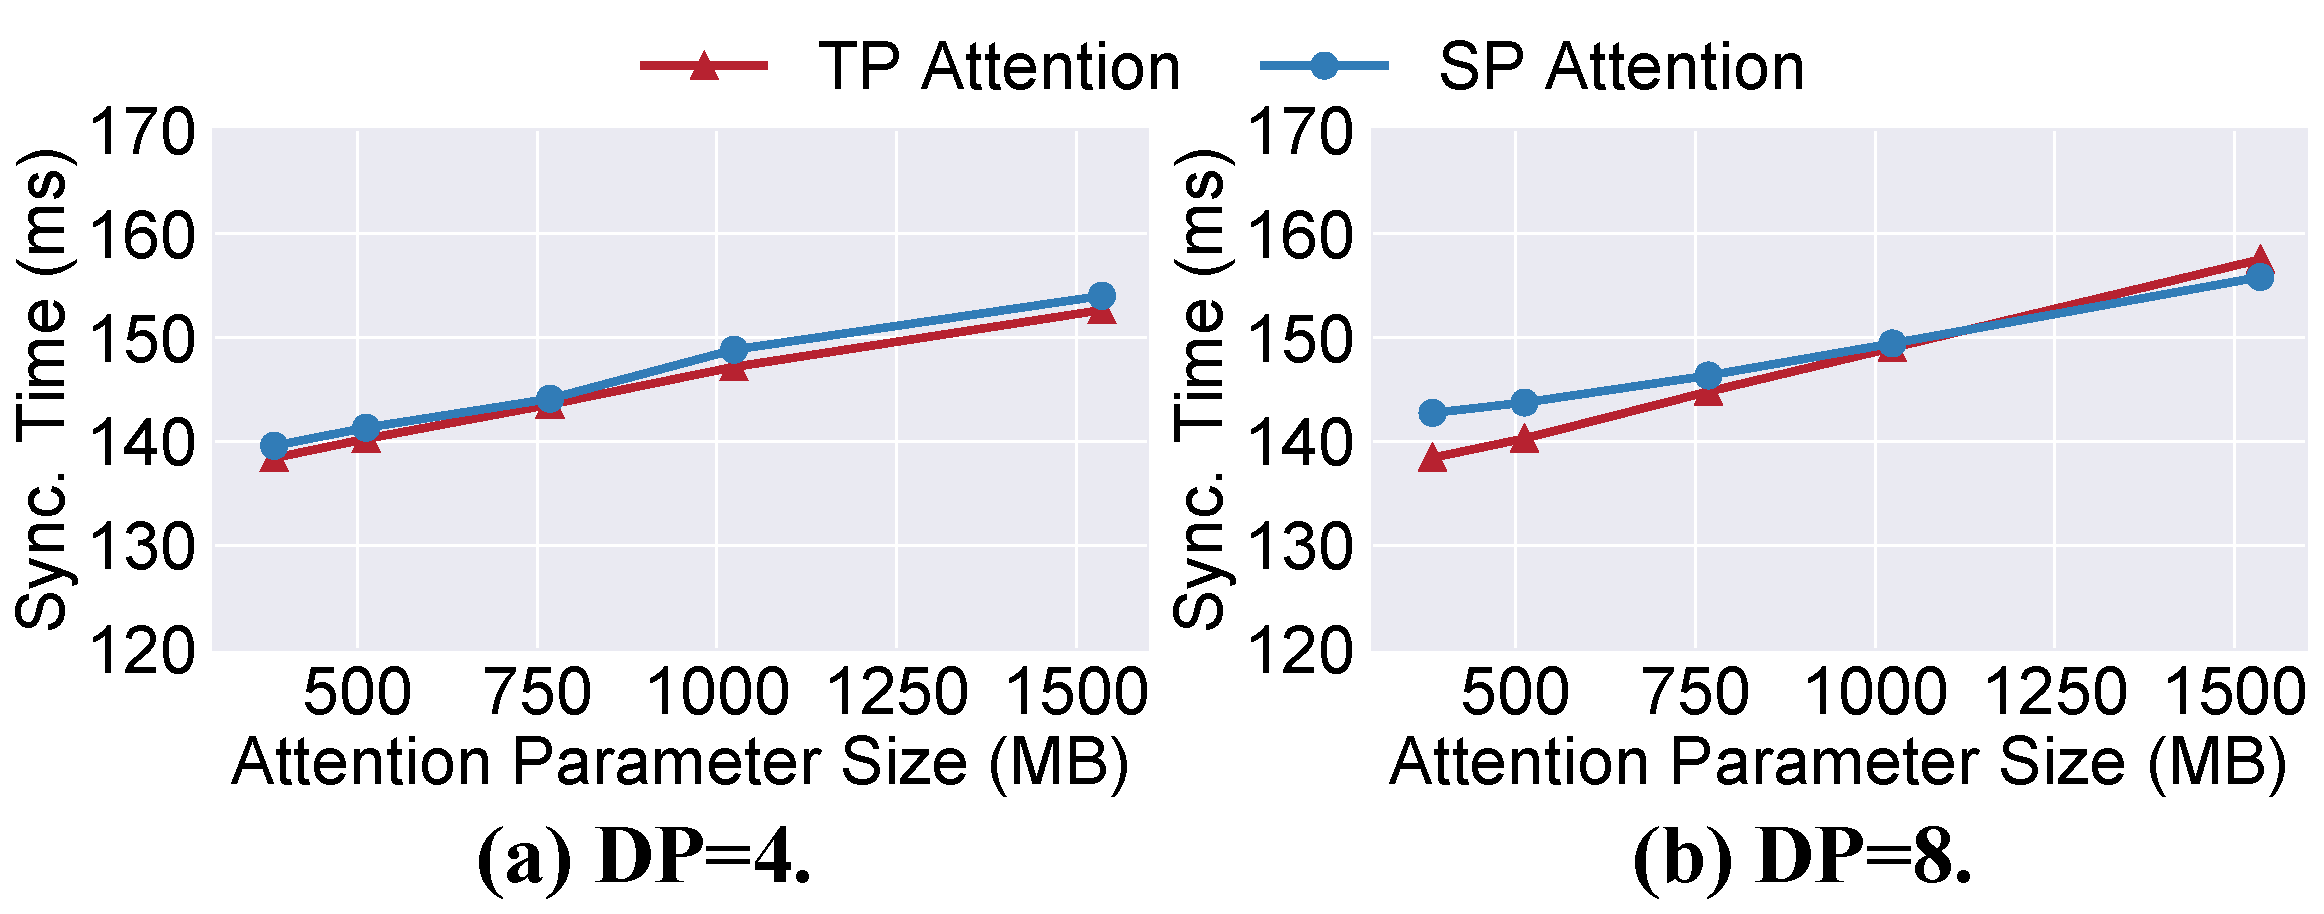
\includegraphics[width=0.9\linewidth]{figures/eval/sync_latency.pdf}
    \vspace{-0.2in}
    \caption{SP 和 TP 注意力下的参数同步时间。}
    \vspace{-0.1in}
    \label{fig:eval:sync_latency}
\end{figure}

\revision{在系统性分解之后，我们对每个组件进行消融研究。每次只改变一个设置，并保持其他设置不变，以更深入理解其行为。}

\begin{figure*}[t!]
    \centering
    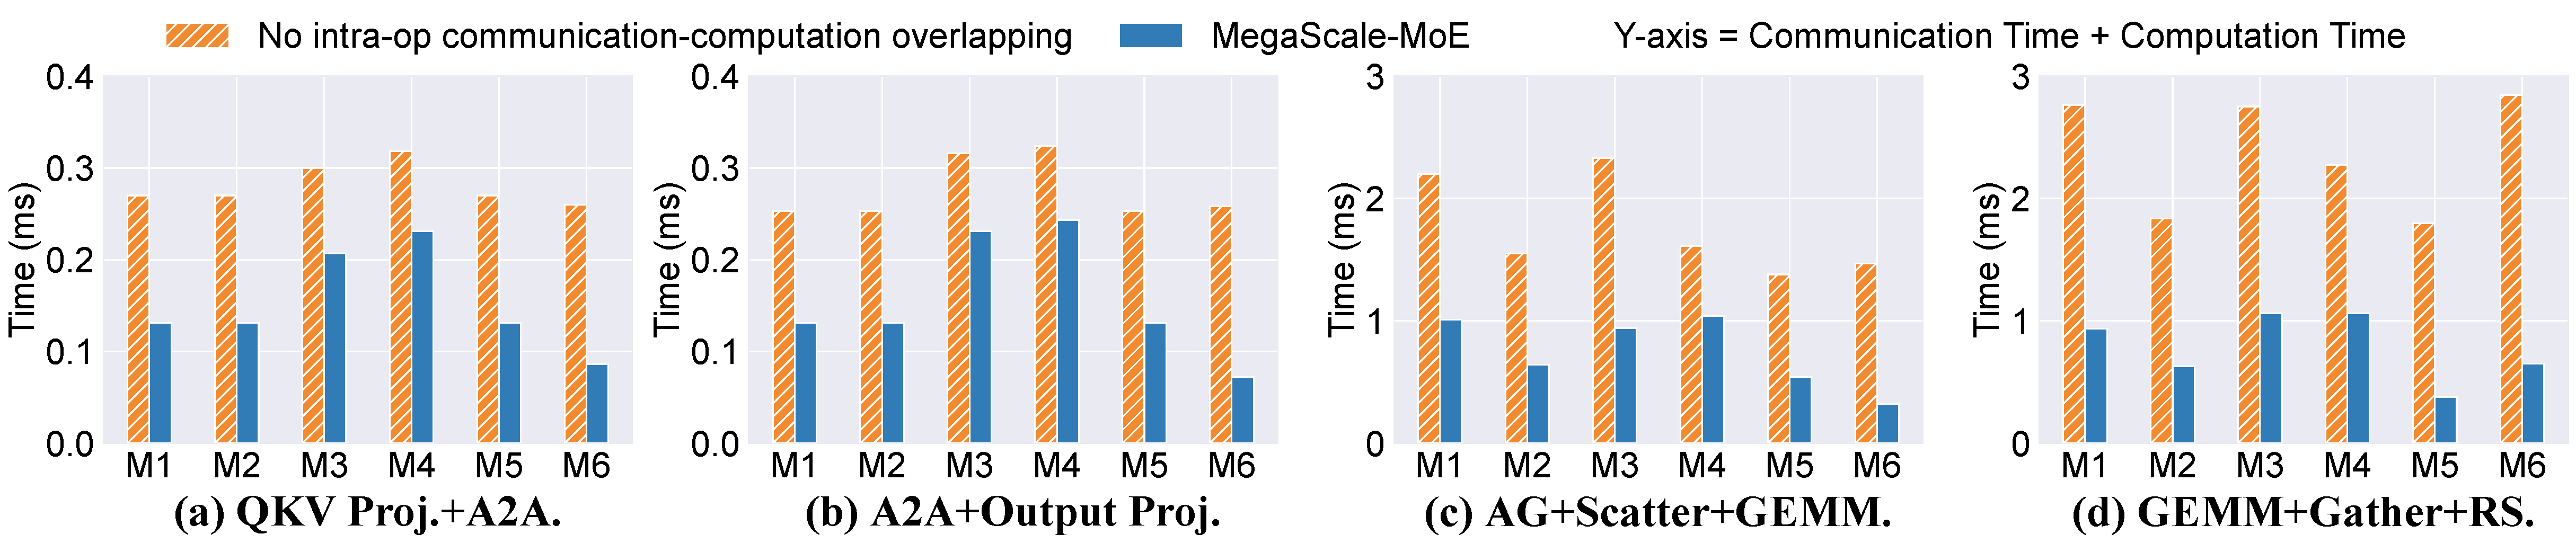
\includegraphics[width=\linewidth]{figures/eval/flux.pdf}
    \vspace{-0.3in}
    \caption{每层中重叠后的通信-计算时间与未重叠时间对比。M1-M6 表示 表~\ref{tab:evaluation:model_conf} 中自上而下列出的六个模型；A2A、AG 和 RS 分别表示 all-to-all、all-gather 和 reduce-scatter。}
    \vspace{-0.1in}
    \label{fig:eval:overlapping}
\end{figure*}

\parabf{并行策略。} 我们使用一个包含 8 张 NVIDIA H800-SXM GPU 的单节点，比较多种节点内并行策略下的训练效率。我们将并行策略记为 X+Y，其中 X 表示注意力的并行策略，Y 表示专家的并行策略。注意力可用的并行策略包括 TP 和我们的 SP，而专家可选 TP 和 EP。为了隔离优化并行带来的性能收益，我们禁用其他系统优化。

\begin{figure}[t!]
    \centering
    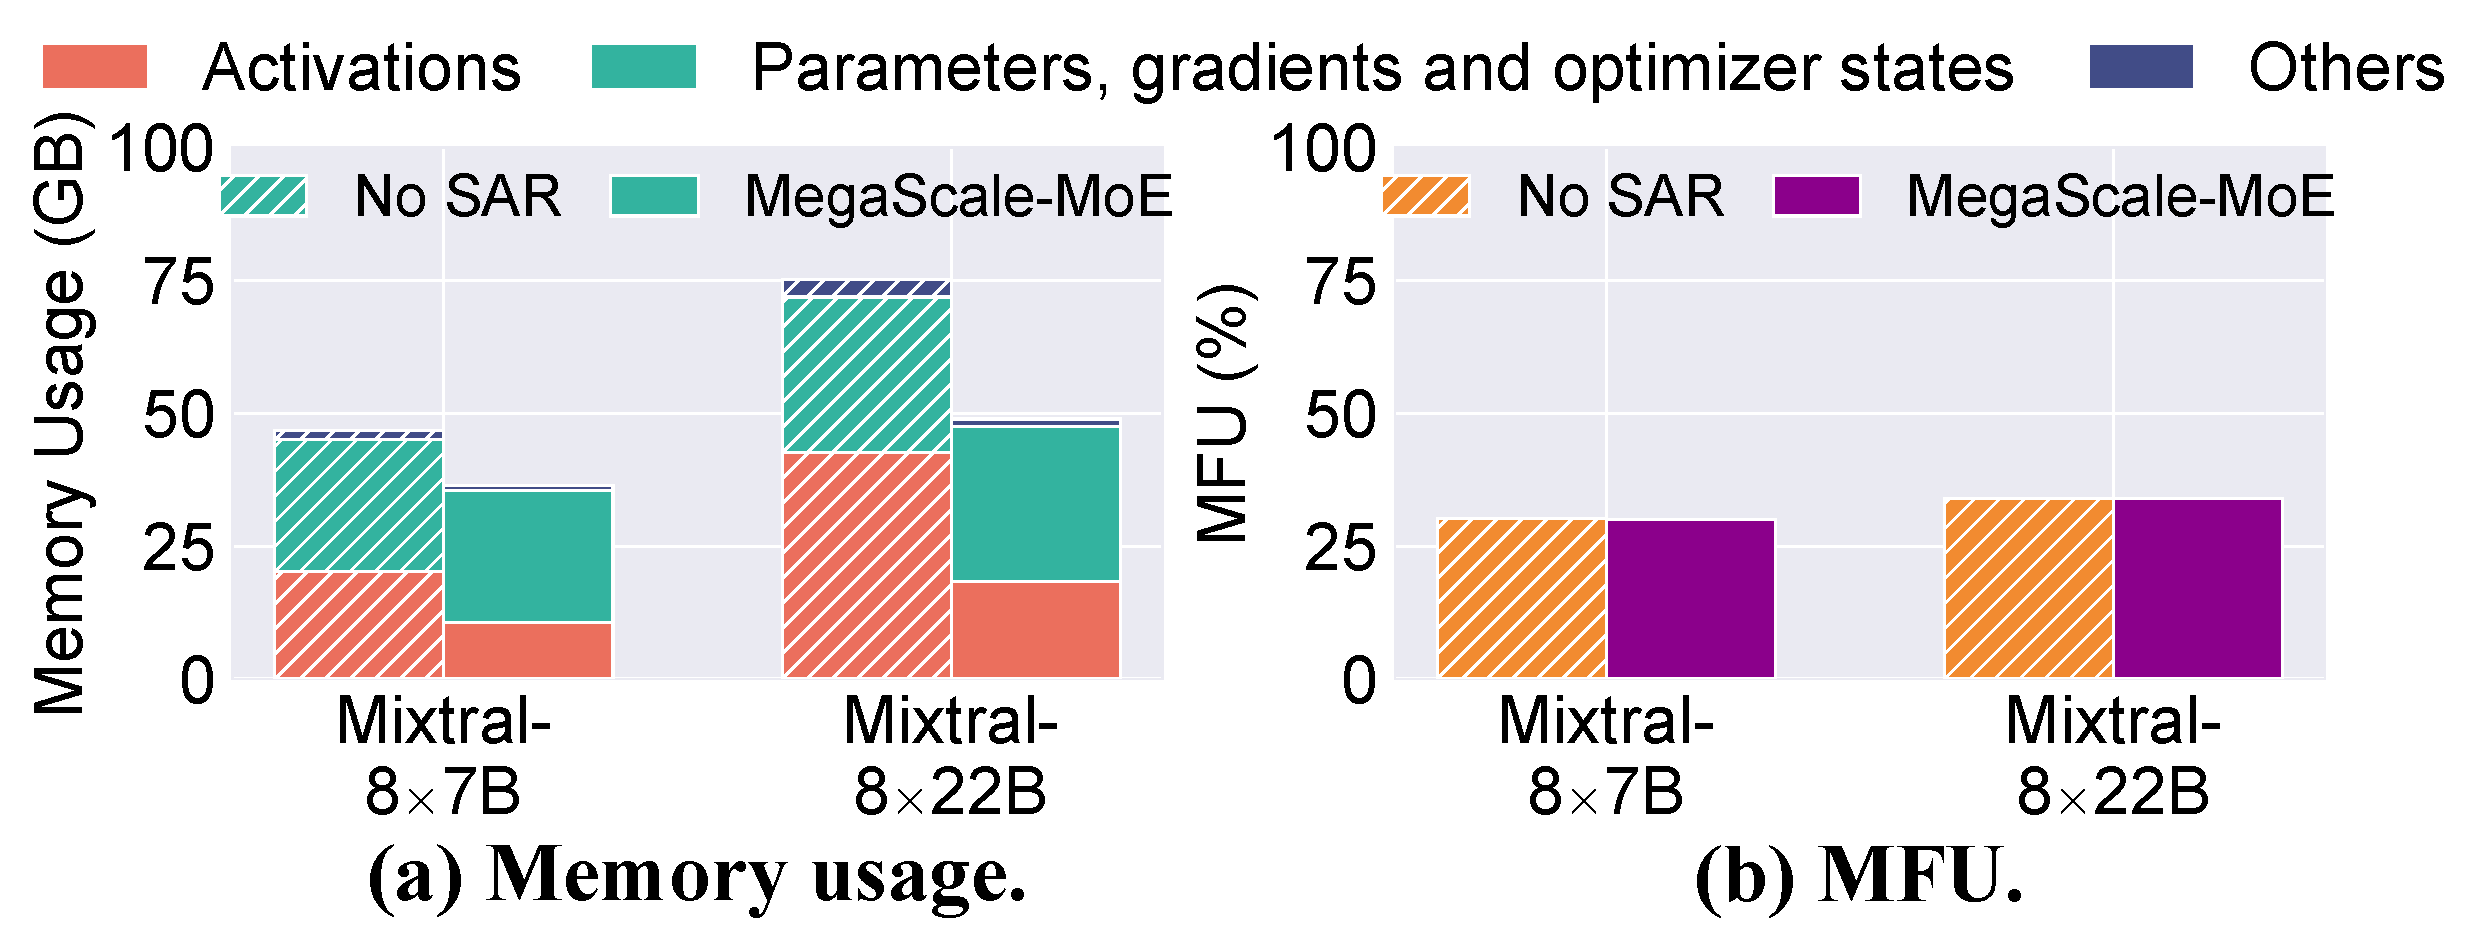
\includegraphics[width=\linewidth]{figures/eval/recomputation.pdf}
    \vspace{-0.3in}
    \caption{选择性激活重物化（SAR）的消融研究。}
    \vspace{-0.1in}
    \label{fig:eval:recompute}
\end{figure}

我们测量了一个内部 MoE 模型和五个开源 MoE 模型的训练 MFU；这些模型具有 表~\ref{tab:evaluation:model_conf} 所列的不同配置。全局 batch size 设为 32，并且我们调整每个模型的层数以适配 GPU 内存。图~\ref{fig:eval:parallelism} 表明，\sysname 的并行策略 SP+EP 始终优于其他三种并行策略，相比 TP+TP 获得 14.9\%--32.9\% 更高 MFU。性能收益归因于两个主要因素。
第一，如 \S\ref{sec:design:parallelism} 所讨论，相比 TP，SP 和 EP 有效减少通信量，从而降低通信开销。第二，TP 沿中间维度切分 FFN 模块，导致 GEMM 效率更低。

为了更全面地评估并行策略，我们还报告了 SP 中复制注意力参数引入的额外开销。在内存使用方面，相比 TP，SP 在全部七个模型上带来 1.2\%--5.4\% 更高的内存占用，并需要多 1.7\%--8.1\% 的内存来存储参数、梯度和优化器状态。考虑到 SP 带来的显著性能收益，这一开销是可控的。
% Besides, in large-scale training with pipeline parallelism, activation memory constitutes a substantial portion of the overall memory footprint, which reduces the impact of replicated attention parameters.

对于参数同步时间，我们遵循大规模训练设置，将 TP 或 SP 的规模设为 8，从而在单节点内有效并行化每一层。
每张 GPU 上的注意力参数大小从 384 MB 变化到 1536 MB，而 FFN 参数大小固定为每张 GPU 10 GB，以反映典型真实训练设置。
我们使用 SP 和 TP attention 运行 \sysname，并使用 4 个和 8 个 DP 组，分别对应总计 32 张和 64 张 GPU。
图~\ref{fig:eval:sync_latency} 表明，SP 和 TP attention 的同步时间始终相当，差异仅为 0.3\%--3.1\%。这与我们的假设一致，即 SP 和 TP 在 DP 通信延迟方面具有相似性能特征。

\parabf{算子内通信重叠。} 接着，我们测量前向传播中四组关键通信及其对应计算算子的耗时：$(i)$ QKV Projection 与 all-to-all，$(ii)$ all-to-all 与 Output Projection，$(iii)$ all-gather 与 scatter 和 GroupedGEMM，$(iv)$ GroupedGEMM 与 gather 和 reduce-scatter，如 图~\ref{fig:moe_computation} 所示。图~\ref{fig:eval:overlapping} 表明，在全部六个模型上，相比缺少细粒度重叠的 baseline，\sysname 将通信和计算算子的总时间降低了 1.2--4.7$\times$。由于算子内通信-计算重叠，\sysname 将训练迭代时间减少了 7.1\%--12.9\%。

\begin{figure}[t!]
    \centering
    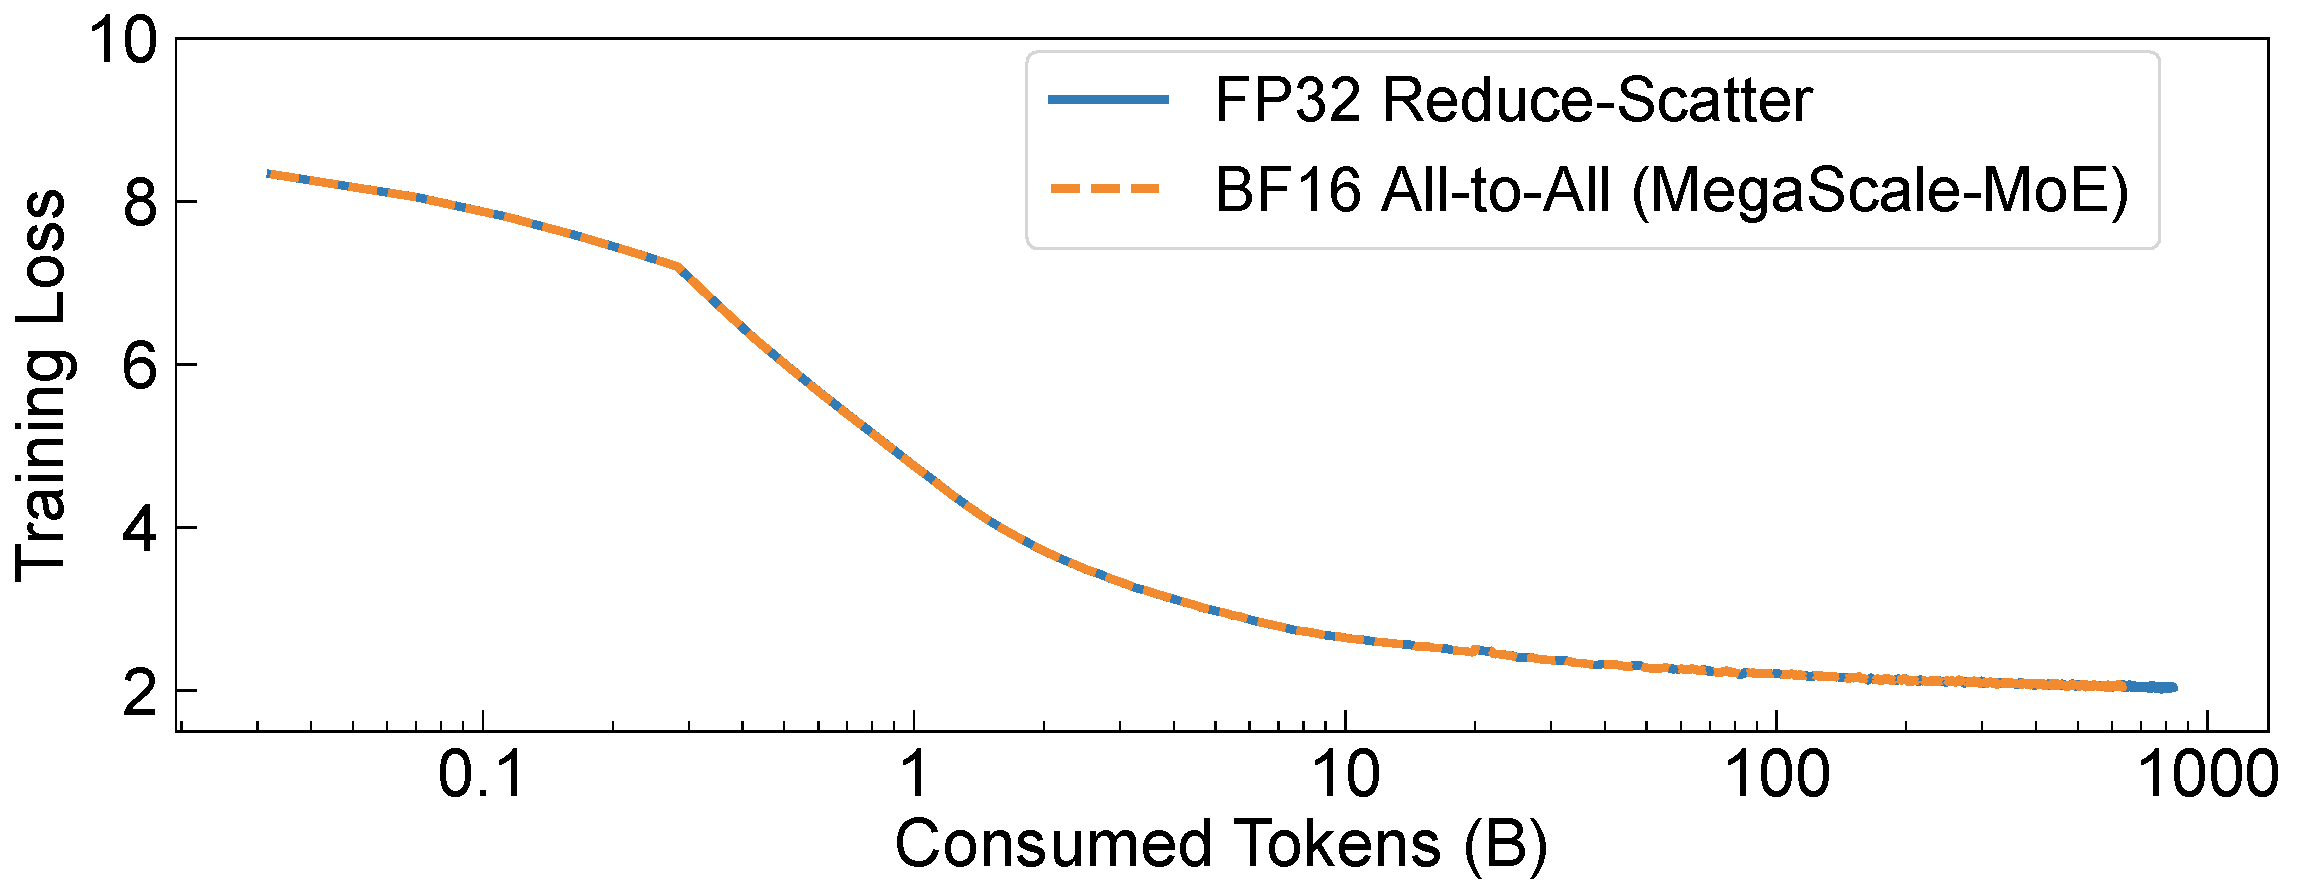
\includegraphics[width=0.8\linewidth]{figures/eval/dp_comm_compression.pdf}
    \vspace{-0.1in}
    \caption{启用 DP 通信压缩时 \sysname 的训练 loss 曲线。}
    \vspace{-0.1in}
    \label{fig:eval:bf16_a2a}
\end{figure}

\parabf{选择性激活重物化。} 我们将 \sysname 与禁用选择性激活重物化（No SAR）的 baseline 进行比较；该 baseline 在训练期间将所有激活都存储在 GPU 内存中。我们在 128 张 NVIDIA H800 GPU 上训练 Mixtral-8$\times$7B 和 Mixtral-8$\times$22B 来评估两种方法。图~\ref{fig:eval:recompute} 展示了内存使用分解和训练 MFU。相比 No SAR，\sysname 分别为两个模型将激活内存消耗降低 45.5\% 和 57.2\%，带来 21.3\% 和 35\% 的整体内存降低，同时将训练性能差异保持在 0.5\% 以内。

\parabf{数据并行通信压缩。} 如 \S\ref{sec:design:precision} 所述，我们通过使用 BF16 all-to-all DP 通信和 FP32 reduce-scatter 通信训练一个 7B MoE 模型，验证通信压缩技术的有效性。图~\ref{fig:eval:bf16_a2a} 展示了几乎完全一致的训练 loss 曲线。该优化只压缩 batch 累加后的梯度，并且只在通信期间执行 BF16 与 FP32 之间的转换，因此风险很小。

\subsection{模型收敛}
\label{sec:evaluation:co-design}

% We evaluate model convergence with our communication compression techniques. 图~\ref{fig:eval:bf16_a2a} compares the training loss curves of \sysname using BF16 all-to-all DP communication and FP32 reduce-scatter communication. The two curves are nearly identical, as this optimization only compresses the gradients of the final micro-batch, posing minimal risk.
% We also validate the effectiveness of FP8 communication compression by training a 25B MoE model from scratch and continuing training a 100B MoE model from a checkpoint, with their loss curves shown in 图~\ref{fig:eval:fp8}. With communication compression and optimizations such as tailored activation quantization, \sysname maintains convergence stability and achieves training loss consistent with the BF16 baseline.

我们评估 \sysname 的模型收敛性。图~\ref{fig:eval:fp8} 展示了从头训练 35B MoE 模型以及从 checkpoint 继续训练 176B MoE 模型的 loss 曲线，并给出了 BF16 和 FP8 两种精度的结果。\sysname 在 BF16 和 FP8 格式下都能保证稳定收敛和一致的训练 loss。

\begin{figure}[t!]
    \centering
    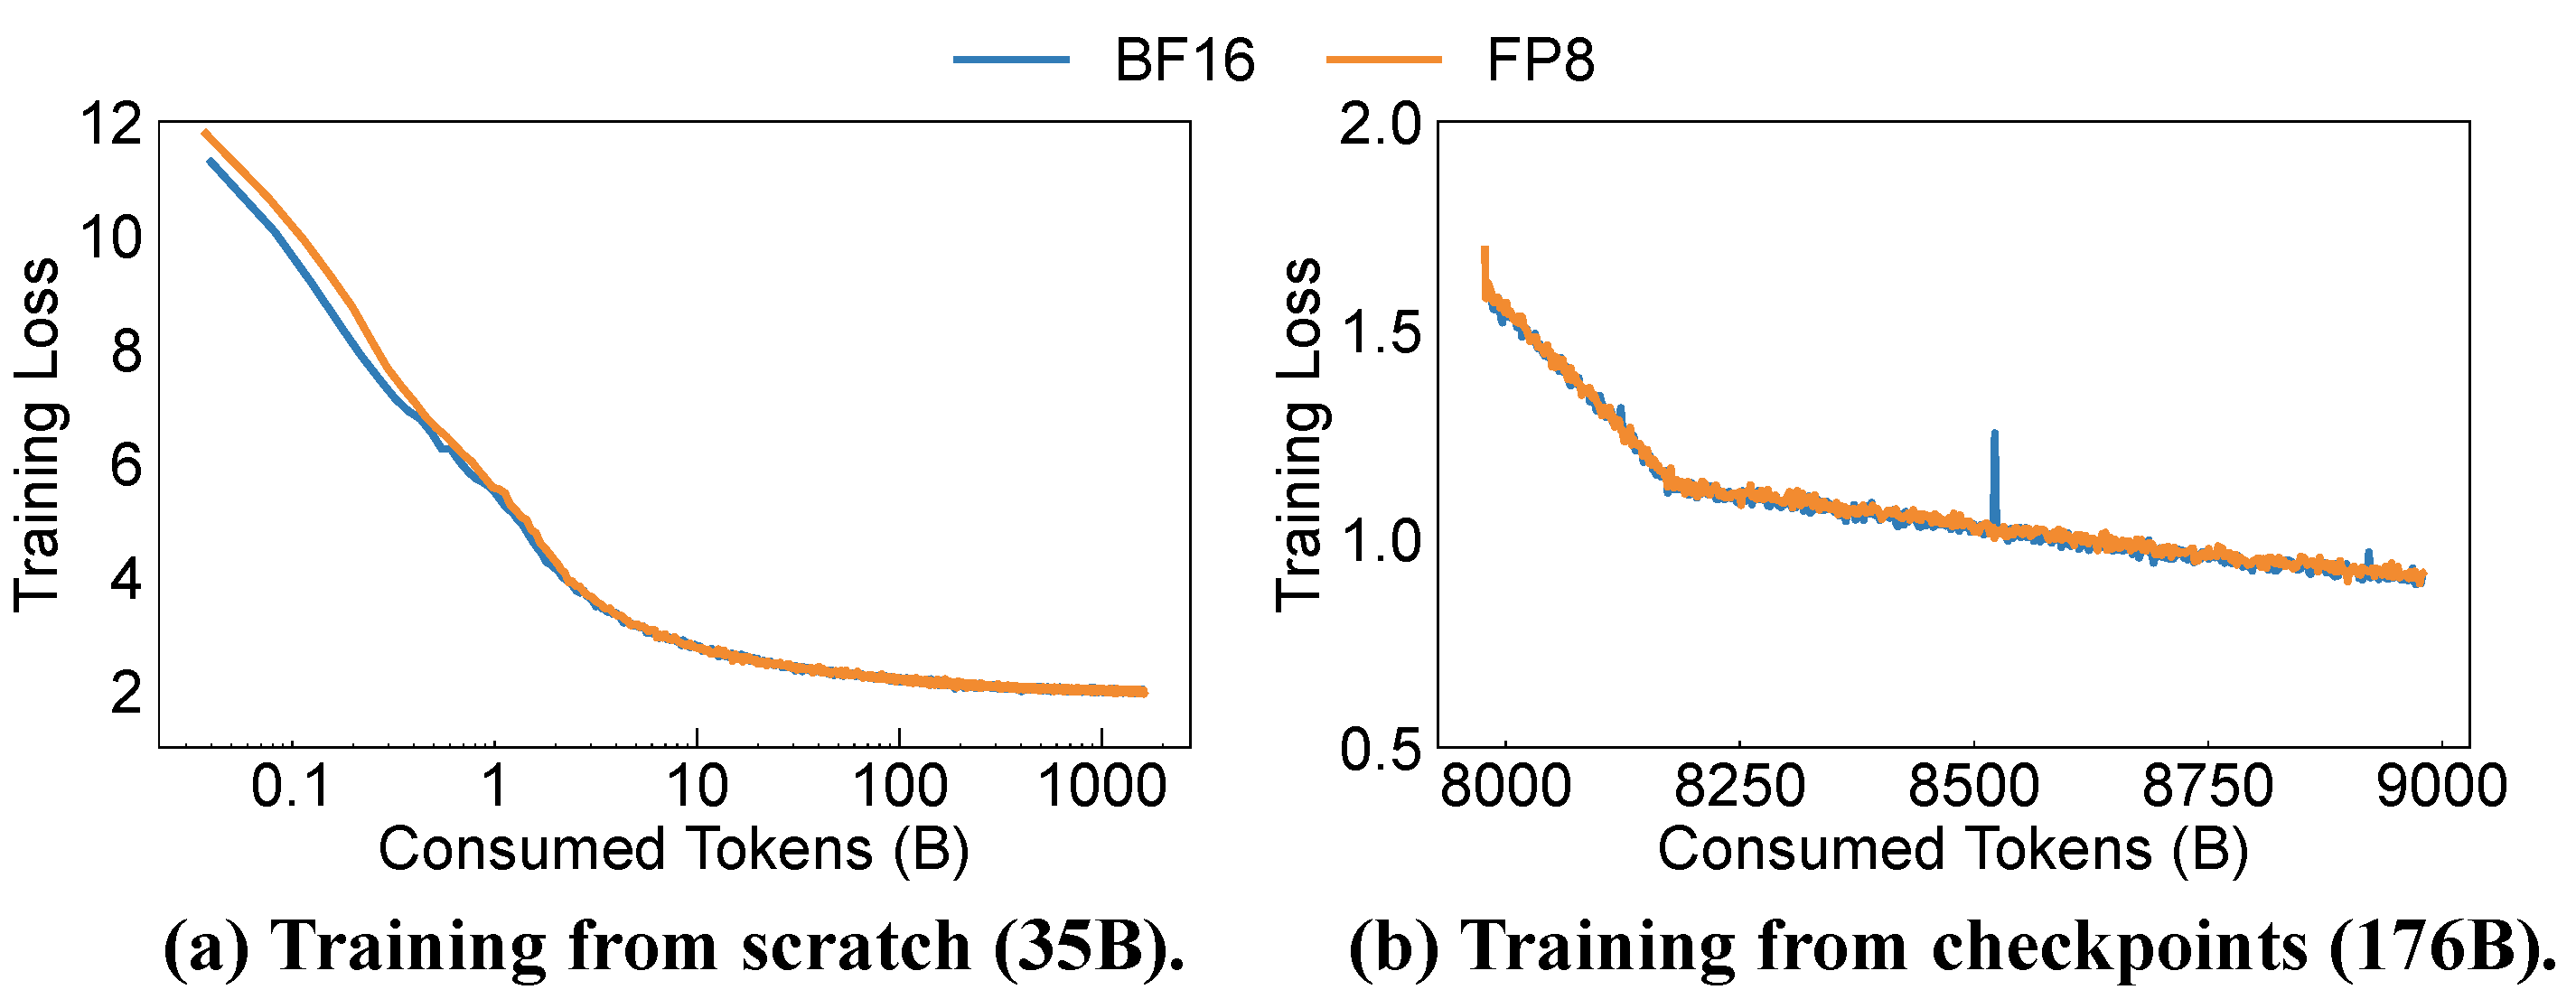
\includegraphics[width=\linewidth]{figures/eval/fp8_comparison.pdf}
    \vspace{-0.2in}
    \caption{\sysname 在 FP8 和 BF16 下的 loss 曲线。}
    \vspace{-0.1in}
    \label{fig:eval:fp8}
\end{figure}
